\section{二次规划}
\label{sec:cone-qp}

拿到一个二次目标、线性约束的问题，于是要问：怎样在动手求解之前，判断它是否凸、解是否唯一、哪些线性代数运算可以直接拿来用？

\paragraph{从带预算的最小二乘开始}
回到章首的三次观测。把三条近似关系写成$\bm{D}\bm{x}\approx\bm{r}$，其中
\[
 \bm{D}=\begin{bmatrix}1&1\\1&0\\0&1\end{bmatrix},\qquad
 \bm{r}=\begin{bmatrix}4\\1\\0\end{bmatrix}.
\]
最小二乘的目标是$\frac12\lVert\bm{D}\bm{x}-\bm{r}\rVert_2^2$，约束是$\bm{x}\geq\bm{0}$和预算$x_1+x_2\leq2$。把这三条约束收集起来，就得到本节贯穿使用的问题。

展开平方，目标等于
\[
 \frac12\bm{x}^\top\bm{D}^\top\bm{D}\bm{x}-\bm{r}^\top\bm{D}\bm{x}+\frac12\lVert\bm{r}\rVert_2^2.
\]
常数项不影响最优解。记$\bm{Q}=\bm{D}^\top\bm{D}$、$\bm{q}=-\bm{D}^\top\bm{r}$，代入数据得到
\begin{equation}
 \bm{Q}=\begin{bmatrix}2&1\\1&2\end{bmatrix},\qquad
 \bm{q}=\begin{bmatrix}-5\\-4\end{bmatrix},\qquad
 \frac12\lVert\bm{r}\rVert_2^2=\frac{17}{2}.
 \label{eq:cone-running-data}
\end{equation}
于是目标是一个对称二次型加一个线性项，约束全是仿射的。

把这种形状抽象出来，就是下面的定义。为了不和最小二乘的$\bm{D},\bm{r}$混淆，约束的系数用另外的字母。

\begin{definition}[二次规划]
\label{def:cone-qp}
设$\bm{Q}\in\mathbb{R}^{n\times n}$对称，$\bm{q}\in\mathbb{R}^n$，$\bm{A}\in\mathbb{R}^{p\times n}$，$\bm{b}\in\mathbb{R}^p$，$\bm{G}\in\mathbb{R}^{m\times n}$，$\bm{h}\in\mathbb{R}^m$。问题
\begin{equation}
 \begin{aligned}
 \min_{\bm{x}\in\mathbb{R}^n}\quad&f(\bm{x})=\frac12\bm{x}^\top\bm{Q}\bm{x}+\bm{q}^\top\bm{x}\\
 \text{s.t.}\quad&\bm{A}\bm{x}=\bm{b},\quad\bm{G}\bm{x}\leq\bm{h}
 \end{aligned}
 \label{eq:cone-qp}
\end{equation}
称为\term{二次规划}（quadratic program，QP）。不等式逐分量理解。可行集$\bm{C}$是有限个闭半空间与超平面的交，即多面体。
\end{definition}

例中$p=0$，三条不等式对应
\[
 \bm{G}=\begin{bmatrix}1&1\\-1&0\\0&-1\end{bmatrix},\qquad
 \bm{h}=\begin{bmatrix}2\\0\\0\end{bmatrix}.
\]
若把预算换成每个分量各自的上下限$\bm{l}\leq\bm{x}\leq\bm{u}$，得到的是盒约束最小二乘，只是$\bm{G},\bm{h}$的内容不同，目标部分完全一样。

\paragraph{拿到二次规划先问三件事}
同一个形式~\eqref{eq:cone-qp}覆盖了难度相差极大的问题，差别由下面三件事决定。

\begin{enumerate}
 \item 曲率：$\bm{Q}$沿可以移动的方向是正、是零还是负？这决定问题是否凸、解是否唯一。
 \item 可行集：有哪些等式和不等式，集合是否有界？这决定解会不会落在边界上、会不会跑到无穷远。
 \item 线性代数结构：$\bm{Q}$和约束矩阵是否稀疏、是否已有分解？这决定一次计算要花多少。
\end{enumerate}

图~\ref{fig:cone-qp-budget}画出例子。蓝色椭圆是目标的等高线，中心$(2,1)$是不考虑约束时的最小二乘解。它的两个分量之和是$3$，超出预算，所以留在三角形内的最好位置落在预算边上。在解$\bm{x}^\star$处，负梯度仍然指向更低的椭圆中心，但沿这个方向走会离开可行集。

\begin{BookInlineFigure}
  \centering
  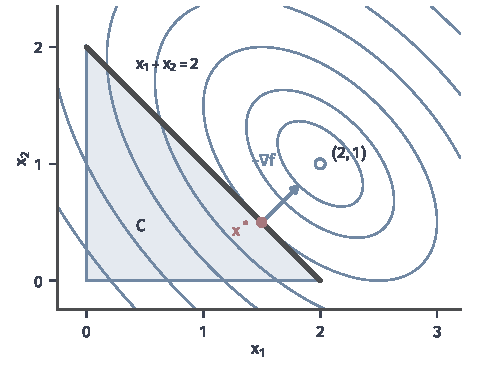
\includegraphics[width=84mm]{figures/05-optimization/06-constrained-optimization/matplotlib/cone-qp-budget/figure.pdf}
  \caption{带预算的最小二乘问题。蓝色椭圆是目标$\frac12\lVert\bm{D}\bm{x}-\bm{r}\rVert_2^2$的等高线，空心点$(2,1)$是无约束解。浅蓝三角形是可行集，深灰粗线是活动的预算约束，红点是解$\bm{x}^\star=(3/2,1/2)$。蓝色箭头是按比例缩短的负梯度，它垂直于预算边。}
  \label{fig:cone-qp-budget}
\end{BookInlineFigure}

\subsection{凸二次规划}
\label{sec:cone-convex-qp}

这一小节回答前两件事：目标在可行集上什么时候是一只碗，这只碗什么时候只有一个最低点。答案全部来自二次函数的一个恒等式。

\paragraph{一个恒等式}
二次函数的特别之处在于，它的高阶余项是零，局部信息就是全局信息。下面的引理把这句话写成精确的等式。

\begin{lemma}[二次函数的两个恒等式]
\label{lem:cone-quadratic-identities}
设$f$是式~\eqref{eq:cone-qp}中的二次函数，$\bm{Q}$对称。则$\nabla f(\bm{x})=\bm{Q}\bm{x}+\bm{q}$，且对任意$\bm{x},\bm{y}\in\mathbb{R}^n$和$\theta\in[0,1]$，
\begin{equation}
 f(\bm{y})=f(\bm{x})+\nabla f(\bm{x})^\top(\bm{y}-\bm{x})+\frac12(\bm{y}-\bm{x})^\top\bm{Q}(\bm{y}-\bm{x}),
 \label{eq:cone-exact-taylor}
\end{equation}
\begin{equation}
 \begin{aligned}
 f(\theta\bm{x}+(1-\theta)\bm{y})={}&\theta f(\bm{x})+(1-\theta)f(\bm{y})\\
 &-\frac12\theta(1-\theta)(\bm{x}-\bm{y})^\top\bm{Q}(\bm{x}-\bm{y}).
 \end{aligned}
 \label{eq:cone-chord-identity}
\end{equation}
\end{lemma}

\begin{proof}
记$\bm{d}=\bm{y}-\bm{x}$。直接展开，
\[
 f(\bm{x}+\bm{d})=\frac12\bm{x}^\top\bm{Q}\bm{x}+\bm{x}^\top\bm{Q}\bm{d}+\frac12\bm{d}^\top\bm{Q}\bm{d}+\bm{q}^\top\bm{x}+\bm{q}^\top\bm{d}.
\]
把含$\bm{d}$一次的两项合并成$(\bm{Q}\bm{x}+\bm{q})^\top\bm{d}$，就是式~\eqref{eq:cone-exact-taylor}。对$\bm{d}$的一次项系数就是梯度。

再证式~\eqref{eq:cone-chord-identity}。令$\bm{d}=\bm{x}-\bm{y}$，则$\theta\bm{x}+(1-\theta)\bm{y}=\bm{y}+\theta\bm{d}$。由式~\eqref{eq:cone-exact-taylor}，
\[
 f(\bm{y}+\theta\bm{d})=f(\bm{y})+\theta\nabla f(\bm{y})^\top\bm{d}+\frac12\theta^2\bm{d}^\top\bm{Q}\bm{d}.
\]
同一公式取步长$1$，得到
\[
 f(\bm{x})=f(\bm{y})+\nabla f(\bm{y})^\top\bm{d}+\frac12\bm{d}^\top\bm{Q}\bm{d}.
\]
于是
\[
 \theta f(\bm{x})+(1-\theta)f(\bm{y})=f(\bm{y})+\theta\nabla f(\bm{y})^\top\bm{d}+\frac12\theta\bm{d}^\top\bm{Q}\bm{d}.
\]
两式相减，差等于$\frac12(\theta^2-\theta)\bm{d}^\top\bm{Q}\bm{d}$，即式~\eqref{eq:cone-chord-identity}最后一项。
\end{proof}

式~\eqref{eq:cone-chord-identity}说，弦上的点比弦下面的函数值高出多少，完全由$(\bm{x}-\bm{y})^\top\bm{Q}(\bm{x}-\bm{y})$决定。线性项在其中不起作用。这一项为正，函数在这条线段上向下弯成碗；为负，则向上拱起。

因此要判断凸性，只需要看$\bm{Q}$在所有“两个可行点之差”上的符号。方向若永远走不到，它的曲率再负也无妨。

\paragraph{只看可行差方向}
把可行差张成的子空间记为
\begin{equation}
 \bm{V}=\operatorname{span}\{\bm{x}-\bm{y}:\bm{x},\bm{y}\in\bm{C}\},
 \label{eq:cone-feasible-subspace}
\end{equation}
并取$\bm{Z}$为一个矩阵，其各列构成$\bm{V}$的基。若$\bm{C}$中存在严格满足全部不等式的点，且$\bm{A}$的约束相容，则$\bm{V}=\ker\bm{A}$；此时$\bm{Z}$就是$\bm{A}$的零空间基。矩阵$\bm{Z}^\top\bm{Q}\bm{Z}$记录了$\bm{Q}$在可行方向上的全部曲率。

\begin{theorem}[可行集上的凸性]
\label{thm:cone-feasible-convexity}
设$\bm{C}$是式~\eqref{eq:cone-qp}的非空可行集，$\bm{Z}$的各列是$\bm{V}$的基。则
\begin{enumerate}
 \item $f$在$\bm{C}$上凸，当且仅当$\bm{Z}^\top\bm{Q}\bm{Z}\succeq\bm{0}$；
 \item $f$在$\bm{C}$上严格凸，当且仅当$\bm{Z}^\top\bm{Q}\bm{Z}\succ\bm{0}$。
\end{enumerate}
特别地，$\bm{Q}\succeq\bm{0}$时$f$在任何凸集上都凸。
\end{theorem}

\begin{proof}
先说明可行差足以探测$\bm{V}$中的每个方向。非空凸集在它的仿射包内有内点，取这样一个点$\bar{\bm{x}}$。存在$\varepsilon>0$，使得对$\bm{V}$中满足$\lVert\bm{d}\rVert_2\leq\varepsilon$的$\bm{d}$，都有$\bar{\bm{x}}+\bm{d}\in\bm{C}$。所以这样的$\bm{d}$是可行差，$\bm{V}$中任一非零方向乘上适当的正数后都是可行差。

设$f$在$\bm{C}$上凸。对$\bm{x}=\bar{\bm{x}}+\bm{d}$和$\bm{y}=\bar{\bm{x}}$，式~\eqref{eq:cone-chord-identity}中的最后一项必须不为正，故$\bm{d}^\top\bm{Q}\bm{d}\geq0$。缩放后对$\bm{V}$中全部方向成立，这就是$\bm{Z}^\top\bm{Q}\bm{Z}\succeq\bm{0}$。

反过来，若$\bm{Z}^\top\bm{Q}\bm{Z}\succeq\bm{0}$，则对任意$\bm{x},\bm{y}\in\bm{C}$，$\bm{x}-\bm{y}\in\bm{V}$，式~\eqref{eq:cone-chord-identity}中的最后一项不为正，$f$在$\bm{C}$上凸。

严格凸的情形相同。取$\bm{x}\neq\bm{y}$和$\theta\in(0,1)$，式~\eqref{eq:cone-chord-identity}说明弦严格高于函数，当且仅当$(\bm{x}-\bm{y})^\top\bm{Q}(\bm{x}-\bm{y})>0$。把上面两段的非负换成严格为正，论证逐句成立。
\end{proof}

最小二乘天然满足定理的条件。对$\bm{Q}=\bm{D}^\top\bm{D}$，有
\[
 \bm{d}^\top\bm{Q}\bm{d}=\lVert\bm{D}\bm{d}\rVert_2^2\geq0.
\]
所以带线性约束的最小二乘总是凸二次规划。严格凸与否取决于$\ker\bm{D}$与$\bm{V}$是否只交于零向量。例中$\bm{D}$列满秩，$\bm{Q}$的特征值是$1$和$3$，全空间正定。

\paragraph{连接线性方程与最优性条件}
没有约束时，最优条件是$\bm{Q}\bm{x}+\bm{q}=\bm{0}$，也就是最小二乘的正规方程$\bm{D}^\top\bm{D}\bm{x}=\bm{D}^\top\bm{r}$，其解法和选解可参考\BookChapterRef{chap:linear-solution-selection}{卷二第11章“线性方程与最小二乘的选解”}。例中由式~\eqref{eq:cone-running-data}解得无约束解$(2,1)$。

加上约束后，方程要换成第~\ref{chap:constrained-optimality}章的KKT条件。那一章证明了：约束全是仿射函数时，局部极小点满足KKT条件，不需要额外的约束规格。对问题~\eqref{eq:cone-qp}，KKT条件写成存在$\bm{\lambda}\in\mathbb{R}^m$和$\bm{\nu}\in\mathbb{R}^p$，使得
\begin{equation}
 \begin{gathered}
 \bm{Q}\bm{x}+\bm{q}+\bm{A}^\top\bm{\nu}+\bm{G}^\top\bm{\lambda}=\bm{0},\\
 \bm{A}\bm{x}=\bm{b},\qquad\bm{G}\bm{x}\leq\bm{h},\\
 \bm{\lambda}\geq\bm{0},\qquad\bm{\lambda}^\top(\bm{G}\bm{x}-\bm{h})=0.
 \end{gathered}
 \label{eq:cone-qp-kkt}
\end{equation}

凸性让这组条件从必要变成充分，也就成了全局最优的证书。

\begin{theorem}[凸二次规划的KKT证书]
\label{thm:cone-qp-kkt}
设$f$在$\bm{C}$上凸。可行点$\bm{x}$是问题~\eqref{eq:cone-qp}的全局最优解，当且仅当存在$\bm{\lambda},\bm{\nu}$使式~\eqref{eq:cone-qp-kkt}成立。
\end{theorem}

\begin{proof}
必要性是上面复述的结论，全局最优解当然是局部极小点。下面证充分性。任取可行点$\bm{y}$，记$\bm{d}=\bm{y}-\bm{x}$。由式~\eqref{eq:cone-exact-taylor}，
\[
 f(\bm{y})-f(\bm{x})=\nabla f(\bm{x})^\top\bm{d}+\frac12\bm{d}^\top\bm{Q}\bm{d}.
\]
$\bm{d}$是可行差，定理~\ref{thm:cone-feasible-convexity}给出$\bm{d}^\top\bm{Q}\bm{d}\geq0$。只需证第一项非负。

把驻定条件代入，并用$\bm{A}\bm{d}=\bm{0}$，得到
\[
 \nabla f(\bm{x})^\top\bm{d}=-\bm{\nu}^\top\bm{A}\bm{d}-\bm{\lambda}^\top\bm{G}\bm{d}=-\bm{\lambda}^\top\bm{G}\bm{d}.
\]
由互补条件$\bm{\lambda}^\top(\bm{G}\bm{x}-\bm{h})=0$，上式可以写成
\[
 -\bm{\lambda}^\top\bm{G}\bm{d}=-\bm{\lambda}^\top(\bm{G}\bm{y}-\bm{h})+\bm{\lambda}^\top(\bm{G}\bm{x}-\bm{h})=-\bm{\lambda}^\top(\bm{G}\bm{y}-\bm{h}).
\]
$\bm{\lambda}\geq\bm{0}$且$\bm{G}\bm{y}\leq\bm{h}$，所以右端非负。于是$f(\bm{y})\geq f(\bm{x})$。
\end{proof}

这个证书的好处是核对便宜。给出$\bm{x}$和$\bm{\lambda}$，只需做几次矩阵乘法，不必重新求解。

\begin{example}[核对预算问题的解]
\label{ex:cone-qp-kkt}
猜测预算活动、非负约束不活动。可行点$(3/2,1/2)$如何得来，下一小节再算，这里先核对。由式~\eqref{eq:cone-running-data}，
\[
 \nabla f(\bm{x})=\bm{Q}\bm{x}+\bm{q}=\begin{bmatrix}7/2\\5/2\end{bmatrix}+\begin{bmatrix}-5\\-4\end{bmatrix}=\begin{bmatrix}-3/2\\-3/2\end{bmatrix}.
\]
取$\bm{\lambda}=(3/2,0,0)$，则
\[
 \nabla f(\bm{x})+\bm{G}^\top\bm{\lambda}=\begin{bmatrix}-3/2\\-3/2\end{bmatrix}+\frac32\begin{bmatrix}1\\1\end{bmatrix}=\bm{0}.
\]
互补条件成立，因为预算的松弛量是$0$，另外两条约束的乘子是$0$。$\bm{\lambda}\geq\bm{0}$也成立。由定理~\ref{thm:cone-qp-kkt}，$(3/2,1/2)$是全局最优解。

最优值按$\frac12\lVert\bm{D}\bm{x}-\bm{r}\rVert_2^2$计算。残差是$\bm{D}\bm{x}-\bm{r}=(-2,1/2,1/2)$，于是
\[
 f^\star=\frac12\Bigl(4+\frac14+\frac14\Bigr)=\frac94.
\]
\end{example}

\paragraph{解的存在与唯一}
凸性不保证最优解存在。$\frac12x_1^2+x_2$的$\bm{Q}$半正定，在全平面上却无下界，沿$x_2\to-\infty$一路下降。有下界时情况好得多：二次函数只要在非空多面体上有下界，就一定取得最小值。这一结论称为Frank--Wolfe定理，它不要求凸性；证明要对约束个数作归纳，处理最小化序列沿回收方向发散的情形，篇幅较长，读者可查阅二次规划方面的专著。

这里有一点值得和一般光滑函数对比。第~\ref{chap:optimization}章的$e^x$在全直线上有下界$0$，却取不到。二次函数不会有这样的渐近行为。

唯一性由曲率直接给出，而且只需要看可行差方向。

\begin{theorem}[存在唯一性的充分条件]
\label{thm:cone-qp-unique}
设$\bm{C}$非空，且对$\bm{V}$中每个非零$\bm{d}$都有$\bm{d}^\top\bm{Q}\bm{d}>0$。则问题~\eqref{eq:cone-qp}恰有一个最优解。
\end{theorem}

\begin{proof}
先证存在。取$\bar{\bm{x}}\in\bm{C}$，$\bm{C}$中的点都可写成$\bar{\bm{x}}+\bm{Z}\bm{u}$。此时$f$成为$\bm{u}$的二次函数，其二次项矩阵$\bm{Z}^\top\bm{Q}\bm{Z}$正定，故$\lVert\bm{u}\rVert_2\to\infty$时函数值趋于$+\infty$，下水平集有界。可行集是闭集，所以下水平集紧，第~\ref{chap:optimization}章的存在定理给出最优解。

再证唯一。设$\bm{x}\neq\bm{y}$都是最优解，中点$\bm{z}=(\bm{x}+\bm{y})/2$可行。对式~\eqref{eq:cone-chord-identity}取$\theta=1/2$，并记$\bm{d}=\bm{x}-\bm{y}\in\bm{V}$，得到
\[
 f(\bm{z})=f^\star-\frac18\bm{d}^\top\bm{Q}\bm{d}<f^\star.
\]
这与$f^\star$是最优值矛盾。
\end{proof}

定理要求的是$\bm{V}$上正定，不是全空间正定。图~\ref{fig:cone-qp-uniqueness}比较了三种情形。

\begin{BookInlineFigure}
  \centering
  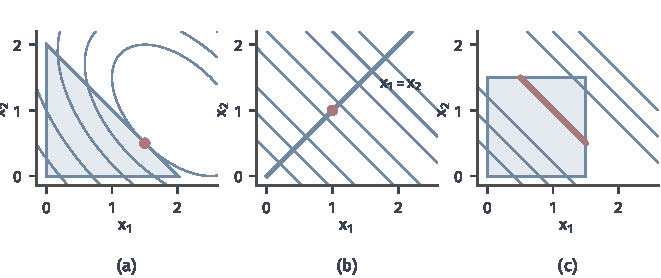
\includegraphics[width=112mm]{figures/05-optimization/06-constrained-optimization/matplotlib/cone-qp-uniqueness/figure.pdf}
  \caption{曲率与解的唯一性，蓝线是目标等高线，红色是解集。(a)预算问题，$\bm{Q}$全空间正定，解唯一。(b)目标$\frac12(x_1+x_2-2)^2$的$\bm{Q}$奇异，等高线是平行直线；约束直线$x_1=x_2$与谷底方向横截，解唯一。(c)同一目标，可行集是正方形$[0,3/2]^2$，平坦方向$(1,-1)$落在可行差内，解集是一条线段。}
  \label{fig:cone-qp-uniqueness}
\end{BookInlineFigure}

(b)中的目标来自只有一次观测的最小二乘，$\bm{D}=\begin{bmatrix}1&1\end{bmatrix}$，$\bm{r}=(2)$，于是$\bm{Q}=\begin{bmatrix}1&1\\1&1\end{bmatrix}$奇异，其零空间由$(1,-1)$张成。约束$x_1=x_2$使$\bm{V}$由$(1,1)$张成，而
\[
 (1,1)\,\bm{Q}\,(1,1)^\top=4>0.
\]
所以在可行直线上目标严格凸，解$(1,1)$唯一。全空间正定不是必要条件。

(c)中可行集仍是平面区域，平坦方向$(1,-1)$属于$\bm{V}$，定理的条件不成立，结论也确实不成立：线段$x_1+x_2=2$上的点全部最优，目标值都是$0$。

$\bm{V}$上正定同样不是唯一性的必要条件。考虑$\frac12x_1^2+x_2$，约束$x_2\geq0$。这里$\bm{V}=\mathbb{R}^2$，方向$(0,1)$的曲率为零，但线性项把解推到边界上：目标在可行集上非负，且只在原点为零，解唯一。线性规划是更极端的情形，$\bm{Q}=\bm{0}$，解却常常是唯一的顶点。

\paragraph{解集与可复用的运算}
凸二次规划的解不唯一时，解集也有规律。设$\bm{x},\bm{y}$都最优，式~\eqref{eq:cone-chord-identity}迫使$\bm{d}^\top\bm{Q}\bm{d}=0$，其中$\bm{d}=\bm{x}-\bm{y}$。$\bm{Q}\succeq\bm{0}$时这又推出$\bm{Q}\bm{d}=\bm{0}$，所以各最优解的梯度相同。解集上变的只有沿平坦方向的位置，不变的是梯度和最优值。

至于第三件事，二次规划的计算几乎都落到线性方程上。$\bm{Q}=\bm{D}^\top\bm{D}$时，$\bm{D}$的QR分解可以反复使用；求解过程换一组活动约束时，只需更新分解，不必重做。求解的形式与代价要到不等式的处理方法确定后才能比较，下一小节先看只有等式的情形。

\subsection{等式约束二次问题}
\label{sec:cone-equality-qp}

假如已经知道哪些不等式在解处活动，把它们当作等式，问题就只剩等式约束。这一小节研究
\begin{equation}
 \min_{\bm{x}}\ \frac12\bm{x}^\top\bm{Q}\bm{x}+\bm{q}^\top\bm{x}\quad\text{s.t.}\quad\bm{A}\bm{x}=\bm{b},
 \label{eq:cone-eqp}
\end{equation}
其中$\bm{A}\in\mathbb{R}^{p\times n}$行满秩，$p<n$。要回答的问题是：它能否化成一次线性方程，什么时候这个方程给出的确实是极小点？

例子取预算恰好用完的情形：$\bm{A}=\begin{bmatrix}1&1\end{bmatrix}$，$b=2$，$\bm{Q},\bm{q}$如式~\eqref{eq:cone-running-data}。可行集是平面上的一条直线。

可行集是一张平的“纸”，有两种自然的处理方式。一种是在纸上另取坐标，把问题变成无约束问题，只看纸面上的碗。另一种是留在原坐标里，引入乘子，把“不许离开纸面”变成方程。

\paragraph{零空间参数化}
取一个特解$\bm{x}_{\mathrm{p}}$满足$\bm{A}\bm{x}_{\mathrm{p}}=\bm{b}$，取$\bm{Z}\in\mathbb{R}^{n\times(n-p)}$，其各列是$\ker\bm{A}$的基。每个可行点都唯一地写成
\begin{equation}
 \bm{x}=\bm{x}_{\mathrm{p}}+\bm{Z}\bm{u},\qquad\bm{u}\in\mathbb{R}^{n-p}.
 \label{eq:cone-nullspace-param}
\end{equation}
约束被消去，$\bm{u}$可以取任意值。

把式~\eqref{eq:cone-nullspace-param}代入目标，并用式~\eqref{eq:cone-exact-taylor}以$\bm{x}_{\mathrm{p}}$为中心展开，得到$\bm{u}$的二次函数
\begin{equation}
 \varphi(\bm{u})=f(\bm{x}_{\mathrm{p}})+\bigl(\bm{Z}^\top(\bm{Q}\bm{x}_{\mathrm{p}}+\bm{q})\bigr)^\top\bm{u}+\frac12\bm{u}^\top\bm{Z}^\top\bm{Q}\bm{Z}\bm{u}.
 \label{eq:cone-reduced-objective}
\end{equation}
矩阵$\bm{Z}^\top\bm{Q}\bm{Z}$称为\term{约化Hessian}（reduced Hessian），它是目标在纸面上的曲率。令梯度为零，得到约化方程
\begin{equation}
 \bm{Z}^\top\bm{Q}\bm{Z}\,\bm{u}=-\bm{Z}^\top(\bm{Q}\bm{x}_{\mathrm{p}}+\bm{q}).
 \label{eq:cone-reduced-equation}
\end{equation}

在例子中取特解$\bm{x}_{\mathrm{p}}=(2,0)$和方向$\bm{z}=(1,-1)$。约化Hessian是一个数：
\[
 \bm{z}^\top\bm{Q}\bm{z}=2-1-1+2=2.
\]
$\bm{x}_{\mathrm{p}}$处的梯度是
\[
 \bm{Q}\bm{x}_{\mathrm{p}}+\bm{q}=\begin{bmatrix}4\\2\end{bmatrix}+\begin{bmatrix}-5\\-4\end{bmatrix}=\begin{bmatrix}-1\\-2\end{bmatrix}.
\]
它在$\bm{z}$上的投影是$\bm{z}^\top(\bm{Q}\bm{x}_{\mathrm{p}}+\bm{q})=1$。把两个数代入式~\eqref{eq:cone-reduced-equation}，得到
\[
 2u=-1,\qquad u^\star=-\frac12.
\]
于是
\[
 \bm{x}^\star=\begin{bmatrix}2\\0\end{bmatrix}-\frac12\begin{bmatrix}1\\-1\end{bmatrix}=\begin{bmatrix}3/2\\1/2\end{bmatrix}.
\]
这个点的两个分量都是正的，所以它也满足原来的非负约束，这正是例~\ref{ex:cone-qp-kkt}核对过的解。

图~\ref{fig:cone-qp-nullspace}(b)画出约化后的一元函数$\varphi(u)=u^2+u+5/2$。原问题的约束已经不见了，剩下的是一个普通的抛物线。

\begin{BookInlineFigure}
  \centering
  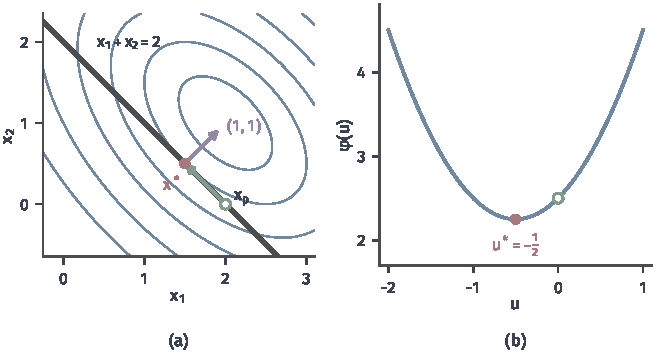
\includegraphics[width=112mm]{figures/05-optimization/06-constrained-optimization/matplotlib/cone-qp-nullspace/figure.pdf}
  \caption{预算恰好用完时的二次问题。(a)深灰粗线是可行直线，蓝线是目标等高线。从特解$\bm{x}_{\mathrm{p}}=(2,0)$（绿色空心点）沿零空间方向走到解（红点），绿色箭头是位移$u^\star\bm{z}$。紫色箭头是约束的法向$(1,1)$，解处的等高线与直线相切，梯度沿这个方向。(b)沿直线的一元函数$\varphi(u)=u^2+u+5/2$，空心点和红点对应(a)中的$\bm{x}_{\mathrm{p}}$与解。}
  \label{fig:cone-qp-nullspace}
\end{BookInlineFigure}

\paragraph{带乘子的块线性方程}
第二种做法不换坐标。对式~\eqref{eq:cone-eqp}写KKT条件，没有不等式，式~\eqref{eq:cone-qp-kkt}只剩两行，它们都是线性的。写成块形式：
\begin{equation}
 \begin{bmatrix}\bm{Q}&\bm{A}^\top\\\bm{A}&\bm{0}\end{bmatrix}
 \begin{bmatrix}\bm{x}\\\bm{\nu}\end{bmatrix}
 =\begin{bmatrix}-\bm{q}\\\bm{b}\end{bmatrix}.
 \label{eq:cone-kkt-system}
\end{equation}
左端的矩阵称为\term{KKT矩阵}（KKT matrix）。它对称，但不定，下方块是零。

例中方程组是
\[
 \begin{bmatrix}2&1&1\\1&2&1\\1&1&0\end{bmatrix}
 \begin{bmatrix}x_1\\x_2\\\nu\end{bmatrix}
 =\begin{bmatrix}5\\4\\2\end{bmatrix}.
\]
前两行相减消去$\nu$，得到$x_1-x_2=1$。第三行给出$x_1+x_2=2$。两式联立，
\[
 x_1=\frac32,\qquad x_2=\frac12.
\]
再代回第一行，
\[
 \nu=5-2x_1-x_2=\frac32.
\]
得到的$\bm{x}$与零空间参数化相同，还多了一个乘子。乘子的含义是预算的影子价格：预算增加一点点，最优值约按$\nu$的速率下降，这种变化率的一般讨论在第~\ref{chap:parametric-sensitivity}章。

两种做法解的是同一组条件。约束$\bm{A}\bm{x}=\bm{b}$由参数化自动满足，而$\ker\bm{A}$的正交补是$\bm{A}^\top$的列空间，所以下面两件事等价：
\begin{equation}
 \bm{Q}\bm{x}+\bm{q}\in\operatorname{range}(\bm{A}^\top)
 \quad\Longleftrightarrow\quad
 \bm{Z}^\top(\bm{Q}\bm{x}+\bm{q})=\bm{0}.
 \label{eq:cone-kkt-reduced-equivalence}
\end{equation}
左边是块方程第一行“存在$\bm{\nu}$”的说法，右边代入式~\eqref{eq:cone-nullspace-param}就是约化方程。

表~\ref{tab:cone-eqp-compare}比较两种做法的计算任务。

\begin{BookInlineTable}
  \centering
  \begin{tabular}{lll}
    \toprule
    & 零空间参数化 & 块线性方程\\
    \midrule
    需要准备 & 特解与零空间基$\bm{Z}$ & 无\\
    解的方程 & $(n-p)$阶，常可用Cholesky & $(n+p)$阶，对称不定\\
    适合的情形 & $n-p$小，$\bm{Z}$易得 & $\bm{Q}$、$\bm{A}$稀疏\\
    副产品 & 乘子需另算 & 直接得到乘子\\
    \bottomrule
  \end{tabular}
  \caption{等式约束二次问题的两种解法。$\bm{Z}$通常来自$\bm{A}^\top$的QR分解，$\bm{Q}$、$\bm{A}$稀疏时$\bm{Z}$和$\bm{Z}^\top\bm{Q}\bm{Z}$可能变稠密。}
  \label{tab:cone-eqp-compare}
\end{BookInlineTable}

\paragraph{唯一可解的条件}
块方程什么时候有唯一解？式~\eqref{eq:cone-kkt-reduced-equivalence}提示答案取决于约化Hessian，而不是$\bm{Q}$本身。

\begin{theorem}[KKT矩阵的可逆性]
\label{thm:cone-kkt-invertible}
设$\bm{A}\in\mathbb{R}^{p\times n}$行满秩，$\bm{Z}$的各列是$\ker\bm{A}$的基。则
\begin{enumerate}
 \item KKT矩阵可逆，当且仅当$\bm{Z}^\top\bm{Q}\bm{Z}$可逆；
 \item 若$\bm{Z}^\top\bm{Q}\bm{Z}\succ\bm{0}$，则式~\eqref{eq:cone-kkt-system}有唯一解，其中的$\bm{x}$是问题~\eqref{eq:cone-eqp}唯一的全局最优解。
\end{enumerate}
\end{theorem}

\begin{proof}
设$(\bm{d},\bm{w})$在KKT矩阵的零空间中，即
\[
 \bm{Q}\bm{d}+\bm{A}^\top\bm{w}=\bm{0},\qquad\bm{A}\bm{d}=\bm{0}.
\]
由第二式可写$\bm{d}=\bm{Z}\bm{u}$。第一式左乘$\bm{Z}^\top$，因为$\bm{A}\bm{Z}=\bm{0}$，得到$\bm{Z}^\top\bm{Q}\bm{Z}\bm{u}=\bm{0}$。

若$\bm{Z}^\top\bm{Q}\bm{Z}$可逆，则$\bm{u}=\bm{0}$，$\bm{d}=\bm{0}$。此时第一式成为$\bm{A}^\top\bm{w}=\bm{0}$，$\bm{A}$行满秩推出$\bm{w}=\bm{0}$。所以KKT矩阵可逆。

反过来，若存在$\bm{u}\neq\bm{0}$使$\bm{Z}^\top\bm{Q}\bm{Z}\bm{u}=\bm{0}$，令$\bm{d}=\bm{Z}\bm{u}\neq\bm{0}$。则$\bm{Q}\bm{d}$与$\ker\bm{A}$正交，属于$\operatorname{range}(\bm{A}^\top)$，存在$\bm{w}$使$\bm{Q}\bm{d}+\bm{A}^\top\bm{w}=\bm{0}$。$(\bm{d},\bm{w})$是非零的零空间向量，KKT矩阵奇异。第一条得证。

第二条的可逆性由第一条给出。此时$\varphi$严格凸，其唯一驻点是唯一的全局极小点；由式~\eqref{eq:cone-kkt-reduced-equivalence}，这个驻点正是块方程解中的$\bm{x}$。
\end{proof}

定理中的“行满秩”也是必需的。若$\bm{A}$行亏秩，存在$\bm{w}\neq\bm{0}$使$\bm{A}^\top\bm{w}=\bm{0}$，$(\bm{0},\bm{w})$就在零空间里，块方程要么无解，要么乘子不唯一。

\paragraph{可逆不等于极小}
线性方程组非奇异，只说明驻点存在且唯一，并不说明驻点是极小点。第一条与第二条之间差的正是约化曲率的符号。

取$\bm{Q}=\operatorname{diag}(1,-1)$，$\bm{q}=\bm{0}$，约束是过原点的直线，方向为$\bm{z}$。图~\ref{fig:cone-qp-reduced}比较了三个方向。目标沿直线$\bm{x}=s\bm{z}$的值是$\frac12s^2\bm{z}^\top\bm{Q}\bm{z}$，约化Hessian就是数$\bm{z}^\top\bm{Q}\bm{z}$。

\begin{BookInlineFigure}
  \centering
  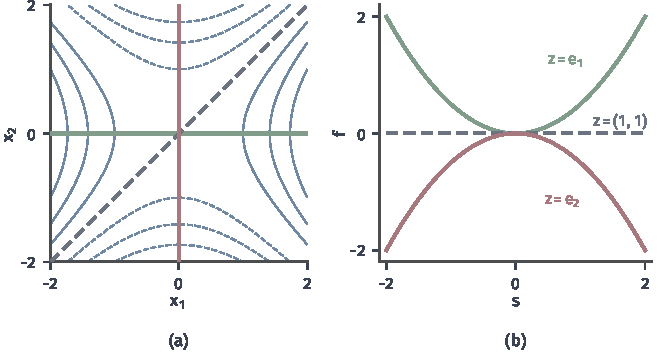
\includegraphics[width=112mm]{figures/05-optimization/06-constrained-optimization/matplotlib/cone-qp-reduced/figure.pdf}
  \caption{约化曲率决定驻点的性质。目标$\frac12(x_1^2-x_2^2)$，$\bm{q}=\bm{0}$。(a)蓝线是等高线（实线为正值，虚线为负值），三条直线是过原点的可行集。(b)目标沿每条直线的取值，横轴是直线上的坐标。绿线的约化曲率为$1$，灰色虚线为$0$，红线为$-1$。}
  \label{fig:cone-qp-reduced}
\end{BookInlineFigure}

表~\ref{tab:cone-reduced-cases}列出三种结果。

\begin{BookInlineTable}
  \centering
  \begin{tabular}{llll}
    \toprule
    方向$\bm{z}$ & $\bm{z}^\top\bm{Q}\bm{z}$ & KKT矩阵 & 原点的性质\\
    \midrule
    $(1,0)$ & $1$ & 可逆 & 唯一全局极小点\\
    $(1,1)$ & $0$ & 奇异 & 整条直线都是驻点\\
    $(0,1)$ & $-1$ & 可逆 & 沿直线的极大点，问题无下界\\
    \bottomrule
  \end{tabular}
  \caption{$\bm{Q}=\operatorname{diag}(1,-1)$、$\bm{q}=\bm{0}$时，约束直线的方向决定KKT矩阵和驻点的性质。}
  \label{tab:cone-reduced-cases}
\end{BookInlineTable}

第三行是要警惕的情形。此时约束是$x_1=0$，$\bm{A}=\begin{bmatrix}1&0\end{bmatrix}$，块方程的矩阵
\[
 \begin{bmatrix}1&0&1\\0&-1&0\\1&0&0\end{bmatrix}
\]
行列式为$1$，可逆，解是$\bm{x}=\bm{0}$、$\nu=0$。求解器不会报告任何异常，但$(0,s)$处的目标是$-\frac12s^2$，$\bm{x}=\bm{0}$是沿可行直线的最高点。

所以解完块方程还要核对约化曲率。不想构造$\bm{Z}$时可以看KKT矩阵的惯性：$\bm{A}$行满秩时，KKT矩阵恰有$n$个正特征值、$p$个负特征值，当且仅当$\bm{Z}^\top\bm{Q}\bm{Z}\succ\bm{0}$，而对称不定分解能直接读出惯性\scite{math-nocedal2006numerical}。

含不等式时，还要决定哪些不等式按等式处理，这个选择问题以及逐步调整的求解方法在第~\ref{chap:sequential-quadratic-programming}章展开。

\subsection{非凸二次问题}
\label{sec:cone-nonconvex-qp}

$\bm{Q}$在可行差方向上有负曲率时，前面的两个定理都不能用。这一小节要弄清：负曲率到底造成什么后果，约束又能挽回多少？

\paragraph{一个负曲率的例子}
考虑$\bm{Q}=\operatorname{diag}(1,-1)$的目标
\begin{equation}
 f(\bm{x})=\frac12x_1^2-\frac12x_2^2+\frac14x_2.
 \label{eq:cone-nonconvex-objective}
\end{equation}
沿$x_1$方向是碗，沿$x_2$方向是倒扣的碗。

先不加约束。唯一的驻点由$x_1=0$和$-x_2+\frac14=0$给出，是$\mathrm{S}=(0,1/4)$。沿$x_2$方向走，目标趋于$-\infty$，所以这个问题无下界，驻点是鞍点。

现在加上$-1\leq x_2\leq1$。约束切断了$x_2$方向的无限下降，$x_1$方向的目标又非负，所以目标在可行集上有下界。这就是图~\ref{fig:cone-qp-nonconvex}(a)中的带形区域。

\begin{BookInlineFigure}
  \centering
  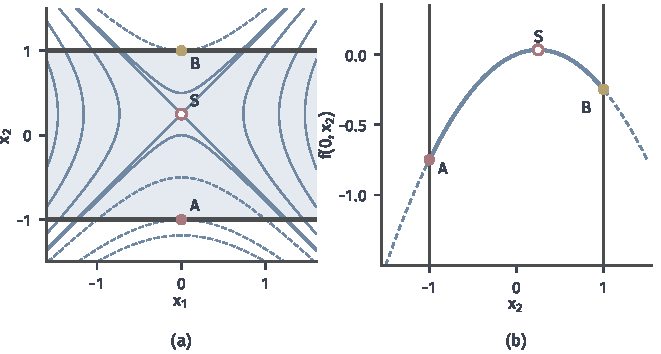
\includegraphics[width=112mm]{figures/05-optimization/06-constrained-optimization/matplotlib/cone-qp-nonconvex/figure.pdf}
  \caption{非凸二次问题的三个KKT点。目标$\frac12x_1^2-\frac12x_2^2+\frac14x_2$，可行集$-1\leq x_2\leq1$。(a)浅蓝带形是可行集，深灰粗线是约束边界，蓝线是等高线（虚线为负的较低水平）。红色实心点A是全局极小点，黄点B是局部极小点，红色空心点S是鞍点。(b)沿$x_1=0$的目标值，两条竖线之外不可行（虚线）。}
  \label{fig:cone-qp-nonconvex}
\end{BookInlineFigure}

\paragraph{KKT点的逐个判别}
约束写成$x_2-1\leq0$和$-x_2-1\leq0$，乘子分别记$\lambda_1,\lambda_2$。驻定条件给出$x_1=0$，以及
\[
 -x_2+\frac14+\lambda_1-\lambda_2=0.
\]
两条约束不能同时活动，所以按活动约束只有三种情形，每一种都是一个线性方程，结果列在表~\ref{tab:cone-nonconvex-kkt}中。

\begin{BookInlineTable}
  \centering
  \begin{tabular}{llll}
    \toprule
    点 & 活动约束 & 乘子 & 目标值\\
    \midrule
    $\mathrm{A}=(0,-1)$ & $x_2\geq-1$ & $\lambda_2=5/4$ & $-3/4$\\
    $\mathrm{B}=(0,1)$ & $x_2\leq1$ & $\lambda_1=3/4$ & $-1/4$\\
    $\mathrm{S}=(0,1/4)$ & 无 & $0$ & $1/32$\\
    \bottomrule
  \end{tabular}
  \caption{目标~\eqref{eq:cone-nonconvex-objective}在带形可行集上的三个KKT点。}
  \label{tab:cone-nonconvex-kkt}
\end{BookInlineTable}

三个点都满足一阶条件，性质却各不相同。判别要用第~\ref{chap:constrained-optimality}章的二阶条件：在乘子为正的活动约束的切方向上看曲率。

在A和B处，活动约束的乘子都为正，临界方向只有$(d_1,0)$，曲率$d_1^2>0$，所以二者都是严格局部极小点。在S处没有活动约束，$\bm{Q}$本身不定，沿$(0,1)$的曲率为负，所以S是鞍点。

比较目标值，A是全局极小点，B只是局部极小点。

\paragraph{不能继承的全局证书}
B满足全部KKT条件，却不是全局最优解。定理~\ref{thm:cone-qp-kkt}的证明在这里断在哪一步？取$\bm{x}=\mathrm{B}$、$\bm{y}=\mathrm{A}$，$\bm{d}=(0,-2)$。式~\eqref{eq:cone-exact-taylor}的两部分分别是
\[
 \nabla f(\mathrm{B})^\top\bm{d}=\Bigl(-\frac34\Bigr)(-2)=\frac32,\qquad
 \frac12\bm{d}^\top\bm{Q}\bm{d}=-2.
\]
一阶部分依然非负，这是KKT条件保证的。但二次部分为负，而且绝对值更大，两者之和是$-1/2$，恰好等于$f(\mathrm{A})-f(\mathrm{B})$。

表~\ref{tab:cone-nonconvex-feasible}把局部最优、鞍点和无下界并列起来。若只保留上界$x_2\leq1$、去掉下界，B依然是严格局部极小点，问题却变成无下界。局部信息看不出全局的命运。

\begin{BookInlineTable}
  \centering
  \begin{tabular}{lll}
    \toprule
    可行集 & 负曲率方向 & 结论\\
    \midrule
    全平面 & 不受限制 & 无下界，S是鞍点\\
    $x_2\leq1$ & 只能向下走 & B局部极小，问题无下界\\
    $-1\leq x_2\leq1$ & 被两侧截断 & A全局极小，B局部极小，S鞍点\\
    $x_2=0$ & 被完全禁止 & 约化后严格凸，解唯一\\
    \bottomrule
  \end{tabular}
  \caption{同一目标~\eqref{eq:cone-nonconvex-objective}在不同可行集上的结果。约束可以限制负曲率方向，但限制的方式决定结论。}
  \label{tab:cone-nonconvex-feasible}
\end{BookInlineTable}

\paragraph{局部解的数量}
局部极小点可以非常多。在盒$[-1,1]^n$上最小化$-\frac12\lVert\bm{x}\rVert_2^2$，每个顶点都是严格局部极小点，共$2^n$个，且每个都满足KKT条件。一般非凸二次规划的全局求解是NP困难问题，这个结论的证明需要计算复杂性理论的归约，这里只用它说明：不能指望靠逐个检查KKT点解决大规模问题。

不过二次结构并没有消失。梯度仍是线性的，每猜一组活动约束仍只需解一次线性方程，局部极小点仍可以用迭代方法找到。缺的是一个能断言“再也找不到更好的点”的全局依据。第~\ref{sec:cone-relax}节将给出另一类下界，用来补上这个缺口。
